% import macros and common styles
\documentclass[11pt]{article}
\usepackage[margin=1in]{geometry}
\usepackage{fancyhdr}
\usepackage[noindentafter]{titlesec}
\usepackage[T1]{fontenc}
\usepackage[scaled]{helvet}
\usepackage[pdftex]{graphicx}
\usepackage{subfigure}
\usepackage[subfigure]{tocloft}
\usepackage{etoc}
\usepackage{float}
\usepackage{amsmath}
\usepackage{amssymb}
\usepackage{changepage}
\usepackage{subfiles}
\usepackage{tabularx}
\usepackage{threeparttable}
\usepackage{caption}
\usepackage{longtable}
\usepackage[table]{xcolor}
\usepackage{tcolorbox}
\usepackage{listings}
\usepackage{color}
\usepackage{hyperref}
\usepackage{keystroke}
\usepackage{wrapfig}
\usepackage{multicol}
\usepackage[table]{xcolor}



\newcommand{\alertbox}[1]{\begin{tcolorbox}[colback=red!5!white,colframe=red!75!black,title=Alert]#1\end{tcolorbox}}


% code block
\definecolor{darkorange}{rgb}{0.99,0.91,0.85}
\definecolor{gray}{rgb}{0.6,0.6,0.6}
\definecolor{darkgray}{rgb}{0.4,0.4,0.4}
\definecolor{white}{rgb}{1,1,1}

\lstset{
	language=C++,
	basicstyle=\fontfamily{NotoSansMono-TLF}\small,
	frame=single,
	showstringspaces=false,
	numbers=none,
	backgroundcolor=\color{darkorange},
	commentstyle=\color{gray},
	linewidth=1\linewidth,
	aboveskip=12pt,
	belowskip=12pt,
	tabsize=4,
	morekeywords={VESSEL, VESSEL2, VESSEL3, VESSEL4, HINSTANCE, OBJHANDLE, FILEHANDLE, PROPELLANT_HANDLE, THRUSTER_HANDLE,
		SURFHANDLE, WORD, DWORD, UINT, HBITMAP, ANIMATIONCOMPONENT_HANDLE, MGROUP_ROTATE, MGROUP_TRANSLATE, MGROUP_SCALE,
		PANELHANDLE, MESHGROUP, NTVERTEX, MFDSPEC, VCMFDSPEC}
}

\lstdefinelanguage{OSFS}{
	basicstyle=\fontfamily{NotoSansMono-TLF}\small\color{white},
	frame=single,
	showstringspaces=false,
	numbers=none,
	backgroundcolor=\color{darkgray},
	commentstyle=\color{darkorange},
	morecomment = [l]{;},
	linewidth=1\linewidth,
	aboveskip=12pt,
	belowskip=12pt,
	tabsize=4,
	keywords = {}
}



\graphicspath{{Images//}}



\renewcommand*\familydefault{\sfdefault}
\sffamily

\pagestyle{fancy}
\renewcommand{\footrulewidth}{0.4pt}


% define page header/footer
\lhead{}
\chead{}
\rhead{}
\lfoot{Atlantis Manual}
\cfoot{\thepage}

\titleformat{\paragraph}[hang]{\bfseries}{\theparagraph}{1em}{}

\begin{document}
\begin{titlepage}
\begin{center}

\vspace*{3.0cm}
\textsc{\fontsize{40}{40} \textbf{Space Shuttle Atlantis}}\\
\vspace{3.0cm}

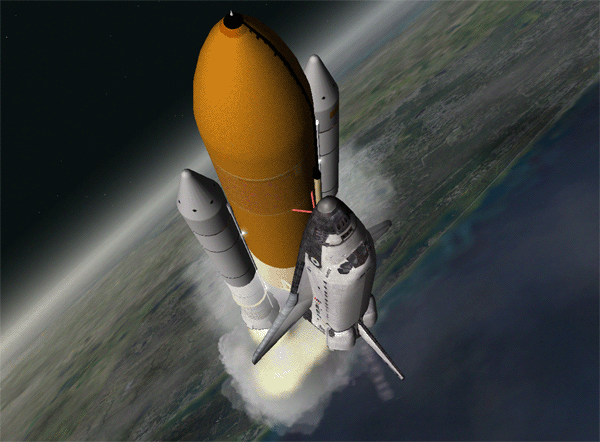
\includegraphics[width=0.75\textwidth]{Images//Pic1.png}
\vspace{2.0cm}

\textsc{\Huge Operations Manual}


\end{center}
\end{titlepage}


\newpage
\pagenumbering{roman}

\tableofcontents
\newpage

\pagenumbering{arabic}

\newcommand{\ks}{\keystroke}
\setlength{\parindent}{0pt}

\newpage
\section{Introduction}
Space Shuttle Atlantis represents the only “real” spacecraft in the basic Orbiter distribution (but there are many more available as add-ons). Its flight characteristics are less forgiving than fictional models like the Delta-glider, and just reaching orbit is a challenge.
The Atlantis orbiter features a working payload bay with remote manipulator system (“Canadarm”), so you can simulate the deployment or even recapture of satellites, or the shipment of resupplies or new modules to the International Space Station.
The model also features a virtual cockpit, including MFD instruments and head-up display.

\section{Virtual cockpit}
You can switch between generic glass cockpit view and virtual cockpit (VC) by pressing \ks{F8}. The virtual cockpit puts you directly on the Atlantis flight deck into the commander’s, pilot’s or payload specialist’s seat, surrounded by display screens and instrument panels. Currently, a subset of instruments is active, including 10 working MFDs, and panel R13L in the rear of the flight deck, controlling the payload door operations.

\begin{center}
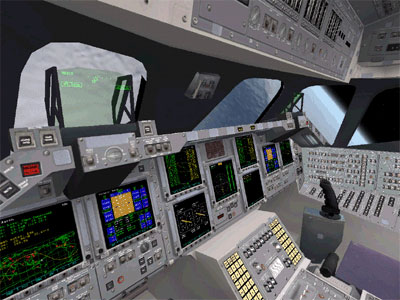
\includegraphics[width=0.75\textwidth]{Images//Pic2.jpg}
\captionof{figure}{The virtual cockpit from the commander’s seat}
\end{center}

\break
\subsection{Navigating the VC}
There are three camera positions available: commander, pilot and payload specialist. By default, you are placed in the commander’s seat, but you can move to a different position by pressing \ks{Ctrl} and an arrow key.  \ks{Ctrl}\ks{$\rightarrow$} and \ks{Ctrl}\ks{$\leftarrow$} jump between the commander and pilot seats, while \ks{Ctrl}\ks{$\downarrow$} switches to and from the payload operator position.\\

\noindent
\textbf{Looking around}\\\

\noindent You can rotate the view at each of the three positions in different ways:
\begin{itemize}
\item by pressing Alt and a cursor key
\item by pressing the right mouse button and dragging the mouse
\item by using the direction controller on the joystick, if available 
\end{itemize}
\vspace{0.5cm}
\noindent
\textbf{Leaning forward and sideways}\\

\noindent
You can also move the head position by pressing \ks{Ctrl}\ks{Alt} in combination with a cursor key. Leaning forward \ks{Ctrl}\ks{Alt}\ks{$\uparrow$} in the commander or pilot position will get you closer to the HUD and instrument panels. Leaning sideways (\ks{Ctrl}\ks{Alt}\ks{$\rightarrow$} and \ks{Ctrl}\ks{Alt}\ks{$\leftarrow$}) provides better access to the MFD instruments on the central panel, or give a better view out of the windows.
In the payload operator position, \ks{Ctrl}\ks{Alt}\ks{$\rightarrow$} provides a view out of the right payload bay window, \ks{Ctrl}\ks{Alt}\ks{$\uparrow$} gets you close to one of the top windows, and \ks{Ctrl}\ks{Alt}\ks{$\leftarrow$} brings the payload door operation panel (R13L) into view.
In all positions, \ks{Ctrl}\ks{Alt}\ks{$\downarrow$} returns to the default head position.

\subsection{Operating the MFDs}
The VC provides 10 multifunctional displays which can be operated independently:
\begin{itemize}
\item 2 commander MFDs (CDR1 and CDR2), accessible from the commander position
\item 2 pilot MFDs (PLT1 and PLT2) accessible from the pilot position
\item 5 MFDs on the central console, accessible from commander and pilot positions
\item 1 MFD on the right rear panel, accessible from the payload operator position
\end{itemize}
Due to the layout of the Shuttle MFD control switches, the operation differs slightly from the generic Orbiter MFD setup. All 10 MFDs work identically. The controls consist of a power button on the left, a brightness dial on the right, and 6 function buttons along the bottom edge.
\begin{itemize} 
\item Clicking the power button turns the MFD on and off.
\item Clicking the left and right half of the brightness button decreases and increases the display brightness, respectively.
\item The left 5 function buttons provide mode-specific functions. The corresponding labels displayed at the bottom of the display change accordingly.
\item The right function button (PG) has a double function: Clicking briefly pages through the function buttons, if the current mode supports more than 5 functions. Holding down the button for longer than one second brings up the mode selection page, with 5 entries per page. You can use the function buttons to select one of the modes.
\end{itemize}
\begin{center}
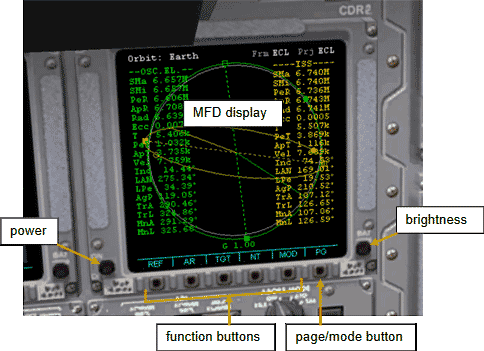
\includegraphics[width=0.75\textwidth]{Images//Pic3.png}
\captionof{figure}{Shuttle MFD screen.}
\end{center}

\section{Notes on operation}
This section contains some details on launch, docking and payload operations of the default Atlantis model distributed with Orbiter. To test the procedures described here in practice, launch Orbiter and try any of the scenarios in the Space Shuttle Atlantis folder.

\subsection{Launch autopilot}
The Space Shuttle needs to follow a tightly defined ascent profile to reach a stable orbit with the available fuel resources, in particular when transporting a heavy payload, or if the mission requires a a high or inclined orbit. You are free to try it manually (unlike the real shuttle), but it is easier (and more realistic) to leave the launch and ascent to the automatic systems.\\

The interface to the ascent autopilot is implemented as an MFD mode (AscentAP, \ks{Shift}\ks{B}). The AP mode has four pages which can be cycled with the 
\texttt{PG-} and \texttt{PG+} buttons. Only the first two pages are currently implemented.\\

Page 1 is the AP configuration page where some of the target orbit parameters can be specified before launch. The launch azimuth angle can be adjusted with the \texttt{AZ-} and \texttt{AZ+} buttons. The selected azimuth, as well as the resulting orbit inclination, are displayed on the page. When launching from Cape Canaveral, the allowed launch azimuth range is 35°–120°, although in practice the Shuttle always launched in north-eastern direction. Remember that the further you deviate from a western (90°) azimuth, the less the trajectory will benefit from Earth’s rotation in terms of initial velocity, and the tighter your fuel budget will be. If the mission calls for a very inclined orbit, you may not be able to load the Shuttle to full payload capacity (30t).\\

The second configurable parameter is the target orbit altitude, adjusted with \texttt{AL-} and \texttt{AL+}. Reaching higher orbits requires more fuel, so if you specify a higher orbit than can be achieved with the available fuel load, the engines will cut out before the trajectory reaches the target apoapsis distance, and there won’t be any reserves for the orbit circularisation burn.\\

Finally, you can schedule or skip the OMS-2 burn. OMS-2 is the second burn of the shuttle orbiter’s OMS (Orbital Maneuvering System) engines. Its purpose is to circularise the orbit once the spacecraft reaches the apoapsis point during ascent. OMS-2 can be commanded to be performed automatically, or you can disable it and then manually perform any required circularisation maneuvers. If the OMS-2 burn is disabled, the AP will disengage at the end of the OMS-1 burn, when the apoapsis distance has reached the commanded orbit altitude.\\ 

\begin{center}
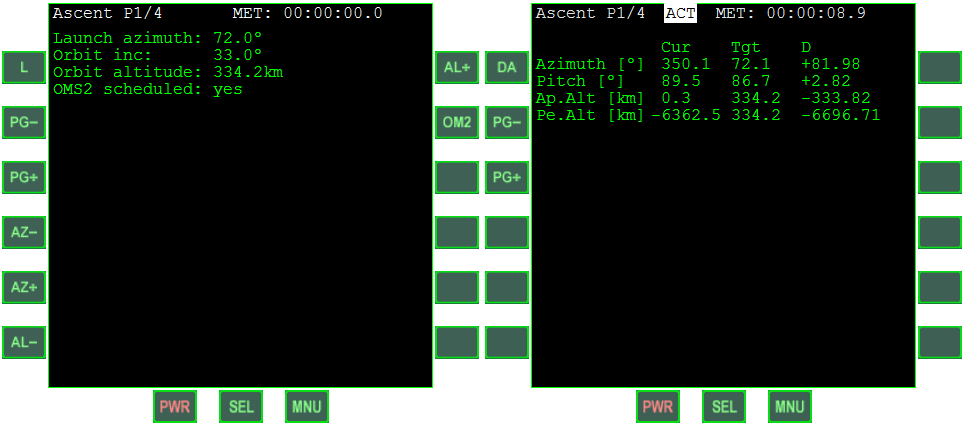
\includegraphics[width=0.75\textwidth]{Images//Pic4.png}
\captionof{figure}{Ascent AP pre-launch configuration page (left) and parameter monitoring page (right).}
\end{center}

Once all launch parameters have been set and the launch window has opened, press L to commence the launch sequence. This will start with the space shuttle main engine (SSME) ignition, and once thrust has stabilised, followed by solid rocket booster (SRB) ignition, and the release of the hold-down bolts.
After lift-off the first page of the AP display switches to monitoring mode, where the target and current values of azimuth, pitch, apoapsis and periapsis altitude are shown as well as the differences.\\

During the first phase of the launch, the stack’s attitude in pitch, yaw and roll is controlled by thrust-vectoring both the SSMEs and the SRB engines. The current gimbal positions of all engines are shown on page 2 of the AP display. The engine mounts allow rotation in both the yaw and pitch axes to provide pitch, yaw and bank moments for the launch stack (while the SRBs are attached, the SSME engines only gimbal in pitch, while the yaw axis is disabled).\\

\begin{center}
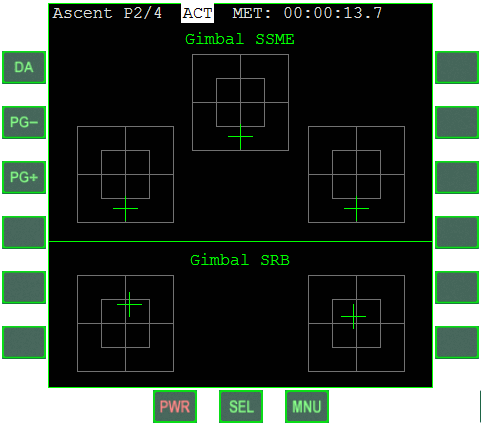
\includegraphics[width=0.75\textwidth]{Images//Pic5.png}
\captionof{figure}{SSME and SRB gimbal monitor.}
\end{center}

After SRB separation, the remaining orbiter + ET (external tank) assembly performs a “rotate upright” maneuver – a rotation of 180° around the longitudinal axis. This is initiated and terminated by a differential pitch gimbal position of the two outer SSMEs.\\

After SSME cut-off and the separation of the ET, attitude control switches to the RCS (reaction control system) – a set of small thrusters engaged in pairs to provide moments around the orbiter’s three axes. These align the orbiter for the OMS-1 burn, using the two OMS engines powered by the on-board fuel supply. The OMS-1 burn commences automatically if the AP is active, and terminates once the apoapsis altitude matches the commanded orbit radius.\\

If the OMS-2 burn was disabled, the AP disengages at this point. Otherwise, the AP waits until the apex of the orbit is reached, then re-aligns the orbiter attitude and fires the OMS engines again to raise periapsis altitude until the orbit is circular with the commanded radius. OMS is cut off and the AP disengages.
You can disengage the AP at any point during the ascent by pressing the DA button on the MFD. This should only be done in an emergency!

\subsection{Manual launch}
You are welcome to ignore the launch autopilot and try to fly the ascent profile manually (a challenge not offered to the real Shuttle pilots). To launch, engage the SSMEs at 100\% thrust (\ks{Num+} and \ks{R-Ctrl} to lock). The SRB engines ignite automatically, the hold-down bolts are blown off, and the launch stack will lift off from the pad. You can control the assembly’s attitude with the normal maneuvering controls (joystick and keyboard, see Orbiter User Manual for details). The pilot’s attitude commands are translated to gimbal deflections of the SSMEs and SRB engines. You can monitor the gimbal positions on page 2 of the ascent autopilot (see previous section). The gimbal information on that page works even when the autopilot is not active. Make sure that the RCS is not activated during ascent. Attitude control during the early flight phase is by thrust-vectoring only.\\

At T + 2:06 minutes (126 seconds after ignition), the SRB fuel is spent and the SRBs detach automatically. In an emergency you can jettison the SRBs early \ks{J}, but in that case you probably also want to jettison the ET (\ks{J} again) and try to return the orbiter to the runway.\\

The following phase of the ascent is flown with the SSMEs only, fed from the ET. As fuel is consumed, the assembly becomes lighter and acceleration increases. Throttle down to keep acceleration at 3g.\\

At T+8:58 minutes, the ET is empty and separates automatically (or can be separated manually before that with j). Altitude at this point should be approximately 110km.\\

After tank separation, the orbiter’s throttle controls now address the OMS engines, fed from internal fuel tanks. Use the initial OMS burn (OMS-1) to push the trajectory apoapsis to the target orbit altitude. Then cut OMS, wait until the Shuttle reaches apoapsis, and fire again prograde (OMS-2) to circularise the orbit. If you flew a good ascent profile, you won’t have run out of fuel yet, and still have enough for the deorbit burn. Otherwise, you are in trouble.\\

\subsection{Docking}
The Shuttle orbiter can carry a docking attachment in the cargo bay. In the real shuttle this was only installed if the mission required docking (e.g. to the ISS), but removed otherwise as it limits payload capacity. In Orbiter, the docking attachment is permanently installed.\\

Prior to docking, the cargo bay doors must be fully open. The docking approach direction is upward as seen from the shuttle orbiter (+y). The Docking MFD mode can be used for linear and rotational alignment, but the relationship between RCS commands and the resulting acceleration axes is different to nose-mounted docking ports and must be considered carefully.

\begin{center}
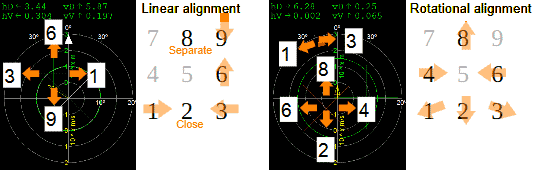
\includegraphics[width=0.75\textwidth]{Images//Pic6.png}
\captionof{figure}{Effect of RCS command input on linear/rotational alignment cues in Docking MFD for Shuttle with docking adapter installed in cargo bay.}
\end{center}






\end{document}